\PassOptionsToPackage{dvipsnames,table}{xcolor}
\documentclass[10pt,french]{beamer}
\usepackage{Cours}

\begin{document}


\newcounter{numchap}
\setcounter{numchap}{1}
\newcounter{numframe}
\setcounter{numframe}{0}
\newcommand{\mframe}[1]{\frametitle{#1} \addtocounter{numframe}{1}}
\newcommand{\cnum}{\fbox{\textcolor{yellow}{\textbf{C\thenumchap}}}~}
\newcommand{\makess}[1]{\section{#1} \label{ss\thesection}}
\newcommand{\stitle}{\textcolor{yellow}{\textbf{\thesection. \nameref{ss\thesection}}}}

\definecolor{codebg}{gray}{0.90}
\definecolor{grispale}{gray}{0.95}
\definecolor{fluo}{rgb}{1,0.96,0.62}
\newminted[langageC]{c}{linenos=true,escapeinside=||,highlightcolor=fluo,tabsize=2,breaklines=true}
\newminted[codepython]{python}{linenos=true,escapeinside=||,highlightcolor=fluo,tabsize=2,breaklines=true}
% Inclusion complète (ou partiel en indiquant premiere et dernière ligne) d'un fichier C
\newcommand{\inputC}[3]{\begin{mdframed}[backgroundcolor=codebg] \inputminted[breaklines=true,fontsize=#3,linenos=true,highlightcolor=fluo,tabsize=2,highlightlines={#2}]{c}{#1} \end{mdframed}}
\newcommand{\inputpartC}[5]{\begin{mdframed}[backgroundcolor=codebg] \inputminted[breaklines=true,fontsize=#3,linenos=true,highlightcolor=fluo,tabsize=2,highlightlines={#2},firstline=#4,lastline=#5,firstnumber=1]{c}{#1} \end{mdframed}}
\newcommand{\inputpython}[3]{\begin{mdframed}[backgroundcolor=codebg] \inputminted[breaklines=true,fontsize=#3,linenos=true,highlightcolor=fluo,tabsize=2,highlightlines={#2}]{python}{#1} \end{mdframed}}
\newcommand{\inputpartOCaml}[5]{\begin{mdframed}[backgroundcolor=codebg] \inputminted[breaklines=true,fontsize=#3,linenos=true,highlightcolor=fluo,tabsize=2,highlightlines={#2},firstline=#4,lastline=#5,firstnumber=1]{OCaml}{#1} \end{mdframed}}
\BeforeBeginEnvironment{minted}{\begin{mdframed}[backgroundcolor=codebg]}
\AfterEndEnvironment{minted}{\end{mdframed}}
\newcommand{\kw}[1]{\textcolor{blue}{\tt #1}}

\newtcolorbox{rcadre}[4]{halign=center,colback={#1},colframe={#2},width={#3cm},height={#4cm},valign=center,boxrule=1pt,left=0pt,right=0pt}
\newtcolorbox{cadre}[4]{halign=center,colback={#1},colframe={#2},arc=0mm,width={#3cm},height={#4cm},valign=center,boxrule=1pt,left=0pt,right=0pt}
\newcommand{\myem}[1]{\colorbox{fluo}{#1}}
\mdfsetup{skipabove=1pt,skipbelow=-2pt}



% Noeud dans un cadre pour les arbres
\newcommand{\noeud}[2]{\Tr{\fbox{\textcolor{#1}{\tt #2}}}}

\newcommand{\htmlmode}{\lstset{language=html,numbers=left, tabsize=4, frame=single, breaklines=true, keywordstyle=\ttfamily, basicstyle=\small,
   numberstyle=\tiny\ttfamily, framexleftmargin=0mm, backgroundcolor=\color{grispale}, xleftmargin=12mm,showstringspaces=false}}
\newcommand{\pythonmode}{\lstset{
   language=python,
   linewidth=\linewidth,
   numbers=left,
   tabsize=4,
   frame=single,
   breaklines=true,
   keywordstyle=\ttfamily\color{blue},
   basicstyle=\small,
   numberstyle=\tiny\ttfamily,
   framexleftmargin=-2mm,
   numbersep=-0.5mm,
   backgroundcolor=\color{codebg},
   xleftmargin=-1mm, 
   showstringspaces=false,
   commentstyle=\color{gray},
   stringstyle=\color{OliveGreen},
   emph={turtle,Screen,Turtle},
   emphstyle=\color{RawSienna},
   morekeywords={setheading,goto,backward,forward,left,right,pendown,penup,pensize,color,speed,hideturtle,showturtle,forward}}
   }
   \newcommand{\Cmode}{\lstset{
      language=[ANSI]C,
      linewidth=\linewidth,
      numbers=left,
      tabsize=4,
      frame=single,
      breaklines=true,
      keywordstyle=\ttfamily\color{blue},
      basicstyle=\small,
      numberstyle=\tiny\ttfamily,
      framexleftmargin=0mm,
      numbersep=2mm,
      backgroundcolor=\color{codebg},
      xleftmargin=0mm, 
      showstringspaces=false,
      commentstyle=\color{gray},
      stringstyle=\color{OliveGreen},
      emphstyle=\color{RawSienna},
      escapechar=\|,
      morekeywords={}}
      }
\newcommand{\bashmode}{\lstset{language=bash,numbers=left, tabsize=2, frame=single, breaklines=true, basicstyle=\ttfamily,
   numberstyle=\tiny\ttfamily, framexleftmargin=0mm, backgroundcolor=\color{grispale}, xleftmargin=12mm, showstringspaces=false}}
\newcommand{\exomode}{\lstset{language=python,numbers=left, tabsize=2, frame=single, breaklines=true, basicstyle=\ttfamily,
   numberstyle=\tiny\ttfamily, framexleftmargin=13mm, xleftmargin=12mm, basicstyle=\small, showstringspaces=false}}
   
   
  
%tei pour placer les images
%tei{nom de l’image}{échelle de l’image}{sens}{texte a positionner}
%sens ="1" (droite) ou "2" (gauche)
\newlength{\ltxt}
\newcommand{\tei}[4]{
\setlength{\ltxt}{\linewidth}
\setbox0=\hbox{\includegraphics[scale=#2]{#1}}
\addtolength{\ltxt}{-\wd0}
\addtolength{\ltxt}{-10pt}
\ifthenelse{\equal{#3}{1}}{
\begin{minipage}{\wd0}
\includegraphics[scale=#2]{#1}
\end{minipage}
\hfill
\begin{minipage}{\ltxt}
#4
\end{minipage}
}{
\begin{minipage}{\ltxt}
#4
\end{minipage}
\hfill
\begin{minipage}{\wd0}
\includegraphics[scale=#2]{#1}
\end{minipage}
}
}

%Juxtaposition d'une image pspciture et de texte 
%#1: = code pstricks de l'image
%#2: largeur de l'image
%#3: hauteur de l'image
%#4: Texte à écrire
\newcommand{\ptp}[4]{
\setlength{\ltxt}{\linewidth}
\addtolength{\ltxt}{-#2 cm}
\addtolength{\ltxt}{-0.1 cm}
\begin{minipage}[b][#3 cm][t]{\ltxt}
#4
\end{minipage}\hfill
\begin{minipage}[b][#3 cm][c]{#2 cm}
#1
\end{minipage}\par
}



%Macros pour les graphiques
\psset{linewidth=0.5\pslinewidth,PointSymbol=x}
\setlength{\fboxrule}{0.5pt}
\newcounter{tempangle}

%Marque la longueur du segment d'extrémité  #1 et  #2 avec la valeur #3, #4 est la distance par rapport au segment (en %age de la valeur de celui ci) et #5 l'orientation du marquage : +90 ou -90
\newcommand{\afflong}[5]{
\pstRotation[RotAngle=#4,PointSymbol=none,PointName=none]{#1}{#2}[X] 
\pstHomO[PointSymbol=none,PointName=none,HomCoef=#5]{#1}{X}[Y]
\pstTranslation[PointSymbol=none,PointName=none]{#1}{#2}{Y}[Z]
 \ncline{|<->|,linewidth=0.25\pslinewidth}{Y}{Z} \ncput*[nrot=:U]{\footnotesize{#3}}
}
\newcommand{\afflongb}[3]{
\ncline{|<->|,linewidth=0}{#1}{#2} \naput*[nrot=:U]{\footnotesize{#3}}
}

%Construis le point #4 situé à #2 cm du point #1 avant un angle #3 par rapport à l'horizontale. #5 = liste de paramètre
\newcommand{\lsegment}[5]{\pstGeonode[PointSymbol=none,PointName=none](0,0){O'}(#2,0){I'} \pstTranslation[PointSymbol=none,PointName=none]{O'}{I'}{#1}[J'] \pstRotation[RotAngle=#3,PointSymbol=x,#5]{#1}{J'}[#4]}
\newcommand{\tsegment}[5]{\pstGeonode[PointSymbol=none,PointName=none](0,0){O'}(#2,0){I'} \pstTranslation[PointSymbol=none,PointName=none]{O'}{I'}{#1}[J'] \pstRotation[RotAngle=#3,PointSymbol=x,#5]{#1}{J'}[#4] \pstLineAB{#4}{#1}}

%Construis le point #4 situé à #3 cm du point #1 et faisant un angle de  90° avec la droite (#1,#2) #5 = liste de paramètre
\newcommand{\psegment}[5]{
\pstGeonode[PointSymbol=none,PointName=none](0,0){O'}(#3,0){I'}
 \pstTranslation[PointSymbol=none,PointName=none]{O'}{I'}{#1}[J']
 \pstInterLC[PointSymbol=none,PointName=none]{#1}{#2}{#1}{J'}{M1}{M2} \pstRotation[RotAngle=-90,PointSymbol=x,#5]{#1}{M1}[#4]
  }
  
%Construis le point #4 situé à #3 cm du point #1 et faisant un angle de  #5° avec la droite (#1,#2) #6 = liste de paramètre
\newcommand{\mlogo}[6]{
\pstGeonode[PointSymbol=none,PointName=none](0,0){O'}(#3,0){I'}
 \pstTranslation[PointSymbol=none,PointName=none]{O'}{I'}{#1}[J']
 \pstInterLC[PointSymbol=none,PointName=none]{#1}{#2}{#1}{J'}{M1}{M2} \pstRotation[RotAngle=#5,PointSymbol=x,#6]{#1}{M2}[#4]
  }

% Construis un triangle avec #1=liste des 3 sommets séparés par des virgules, #2=liste des 3 longueurs séparés par des virgules, #3 et #4 : paramètre d'affichage des 2e et 3 points et #5 : inclinaison par rapport à l'horizontale
%autre macro identique mais sans tracer les segments joignant les sommets
\noexpandarg
\newcommand{\Triangleccc}[5]{
\StrBefore{#1}{,}[\pointA]
\StrBetween[1,2]{#1}{,}{,}[\pointB]
\StrBehind[2]{#1}{,}[\pointC]
\StrBefore{#2}{,}[\coteA]
\StrBetween[1,2]{#2}{,}{,}[\coteB]
\StrBehind[2]{#2}{,}[\coteC]
\tsegment{\pointA}{\coteA}{#5}{\pointB}{#3} 
\lsegment{\pointA}{\coteB}{0}{Z1}{PointSymbol=none, PointName=none}
\lsegment{\pointB}{\coteC}{0}{Z2}{PointSymbol=none, PointName=none}
\pstInterCC{\pointA}{Z1}{\pointB}{Z2}{\pointC}{Z3} 
\pstLineAB{\pointA}{\pointC} \pstLineAB{\pointB}{\pointC}
\pstSymO[PointName=\pointC,#4]{C}{C}[C]
}
\noexpandarg
\newcommand{\TrianglecccP}[5]{
\StrBefore{#1}{,}[\pointA]
\StrBetween[1,2]{#1}{,}{,}[\pointB]
\StrBehind[2]{#1}{,}[\pointC]
\StrBefore{#2}{,}[\coteA]
\StrBetween[1,2]{#2}{,}{,}[\coteB]
\StrBehind[2]{#2}{,}[\coteC]
\tsegment{\pointA}{\coteA}{#5}{\pointB}{#3} 
\lsegment{\pointA}{\coteB}{0}{Z1}{PointSymbol=none, PointName=none}
\lsegment{\pointB}{\coteC}{0}{Z2}{PointSymbol=none, PointName=none}
\pstInterCC[PointNameB=none,PointSymbolB=none,#4]{\pointA}{Z1}{\pointB}{Z2}{\pointC}{Z1} 
}


% Construis un triangle avec #1=liste des 3 sommets séparés par des virgules, #2=liste formée de 2 longueurs et d'un angle séparés par des virgules, #3 et #4 : paramètre d'affichage des 2e et 3 points et #5 : inclinaison par rapport à l'horizontale
%autre macro identique mais sans tracer les segments joignant les sommets
\newcommand{\Trianglecca}[5]{
\StrBefore{#1}{,}[\pointA]
\StrBetween[1,2]{#1}{,}{,}[\pointB]
\StrBehind[2]{#1}{,}[\pointC]
\StrBefore{#2}{,}[\coteA]
\StrBetween[1,2]{#2}{,}{,}[\coteB]
\StrBehind[2]{#2}{,}[\angleA]
\tsegment{\pointA}{\coteA}{#5}{\pointB}{#3} 
\setcounter{tempangle}{#5}
\addtocounter{tempangle}{\angleA}
\tsegment{\pointA}{\coteB}{\thetempangle}{\pointC}{#4}
\pstLineAB{\pointB}{\pointC}
}
\newcommand{\TriangleccaP}[5]{
\StrBefore{#1}{,}[\pointA]
\StrBetween[1,2]{#1}{,}{,}[\pointB]
\StrBehind[2]{#1}{,}[\pointC]
\StrBefore{#2}{,}[\coteA]
\StrBetween[1,2]{#2}{,}{,}[\coteB]
\StrBehind[2]{#2}{,}[\angleA]
\lsegment{\pointA}{\coteA}{#5}{\pointB}{#3} 
\setcounter{tempangle}{#5}
\addtocounter{tempangle}{\angleA}
\lsegment{\pointA}{\coteB}{\thetempangle}{\pointC}{#4}
}

% Construis un triangle avec #1=liste des 3 sommets séparés par des virgules, #2=liste formée de 1 longueurs et de deux angle séparés par des virgules, #3 et #4 : paramètre d'affichage des 2e et 3 points et #5 : inclinaison par rapport à l'horizontale
%autre macro identique mais sans tracer les segments joignant les sommets
\newcommand{\Trianglecaa}[5]{
\StrBefore{#1}{,}[\pointA]
\StrBetween[1,2]{#1}{,}{,}[\pointB]
\StrBehind[2]{#1}{,}[\pointC]
\StrBefore{#2}{,}[\coteA]
\StrBetween[1,2]{#2}{,}{,}[\angleA]
\StrBehind[2]{#2}{,}[\angleB]
\tsegment{\pointA}{\coteA}{#5}{\pointB}{#3} 
\setcounter{tempangle}{#5}
\addtocounter{tempangle}{\angleA}
\lsegment{\pointA}{1}{\thetempangle}{Z1}{PointSymbol=none, PointName=none}
\setcounter{tempangle}{#5}
\addtocounter{tempangle}{180}
\addtocounter{tempangle}{-\angleB}
\lsegment{\pointB}{1}{\thetempangle}{Z2}{PointSymbol=none, PointName=none}
\pstInterLL[#4]{\pointA}{Z1}{\pointB}{Z2}{\pointC}
\pstLineAB{\pointA}{\pointC}
\pstLineAB{\pointB}{\pointC}
}
\newcommand{\TrianglecaaP}[5]{
\StrBefore{#1}{,}[\pointA]
\StrBetween[1,2]{#1}{,}{,}[\pointB]
\StrBehind[2]{#1}{,}[\pointC]
\StrBefore{#2}{,}[\coteA]
\StrBetween[1,2]{#2}{,}{,}[\angleA]
\StrBehind[2]{#2}{,}[\angleB]
\lsegment{\pointA}{\coteA}{#5}{\pointB}{#3} 
\setcounter{tempangle}{#5}
\addtocounter{tempangle}{\angleA}
\lsegment{\pointA}{1}{\thetempangle}{Z1}{PointSymbol=none, PointName=none}
\setcounter{tempangle}{#5}
\addtocounter{tempangle}{180}
\addtocounter{tempangle}{-\angleB}
\lsegment{\pointB}{1}{\thetempangle}{Z2}{PointSymbol=none, PointName=none}
\pstInterLL[#4]{\pointA}{Z1}{\pointB}{Z2}{\pointC}
}

%Construction d'un cercle de centre #1 et de rayon #2 (en cm)
\newcommand{\Cercle}[2]{
\lsegment{#1}{#2}{0}{Z1}{PointSymbol=none, PointName=none}
\pstCircleOA{#1}{Z1}
}

%construction d'un parallélogramme #1 = liste des sommets, #2 = liste contenant les longueurs de 2 côtés consécutifs et leurs angles;  #3, #4 et #5 : paramètre d'affichage des sommets #6 inclinaison par rapport à l'horizontale 
% meme macro sans le tracé des segements
\newcommand{\Para}[6]{
\StrBefore{#1}{,}[\pointA]
\StrBetween[1,2]{#1}{,}{,}[\pointB]
\StrBetween[2,3]{#1}{,}{,}[\pointC]
\StrBehind[3]{#1}{,}[\pointD]
\StrBefore{#2}{,}[\longueur]
\StrBetween[1,2]{#2}{,}{,}[\largeur]
\StrBehind[2]{#2}{,}[\angle]
\tsegment{\pointA}{\longueur}{#6}{\pointB}{#3} 
\setcounter{tempangle}{#6}
\addtocounter{tempangle}{\angle}
\tsegment{\pointA}{\largeur}{\thetempangle}{\pointD}{#5}
\pstMiddleAB[PointName=none,PointSymbol=none]{\pointB}{\pointD}{Z1}
\pstSymO[#4]{Z1}{\pointA}[\pointC]
\pstLineAB{\pointB}{\pointC}
\pstLineAB{\pointC}{\pointD}
}
\newcommand{\ParaP}[6]{
\StrBefore{#1}{,}[\pointA]
\StrBetween[1,2]{#1}{,}{,}[\pointB]
\StrBetween[2,3]{#1}{,}{,}[\pointC]
\StrBehind[3]{#1}{,}[\pointD]
\StrBefore{#2}{,}[\longueur]
\StrBetween[1,2]{#2}{,}{,}[\largeur]
\StrBehind[2]{#2}{,}[\angle]
\lsegment{\pointA}{\longueur}{#6}{\pointB}{#3} 
\setcounter{tempangle}{#6}
\addtocounter{tempangle}{\angle}
\lsegment{\pointA}{\largeur}{\thetempangle}{\pointD}{#5}
\pstMiddleAB[PointName=none,PointSymbol=none]{\pointB}{\pointD}{Z1}
\pstSymO[#4]{Z1}{\pointA}[\pointC]
}


%construction d'un cerf-volant #1 = liste des sommets, #2 = liste contenant les longueurs de 2 côtés consécutifs et leurs angles;  #3, #4 et #5 : paramètre d'affichage des sommets #6 inclinaison par rapport à l'horizontale 
% meme macro sans le tracé des segements
\newcommand{\CerfVolant}[6]{
\StrBefore{#1}{,}[\pointA]
\StrBetween[1,2]{#1}{,}{,}[\pointB]
\StrBetween[2,3]{#1}{,}{,}[\pointC]
\StrBehind[3]{#1}{,}[\pointD]
\StrBefore{#2}{,}[\longueur]
\StrBetween[1,2]{#2}{,}{,}[\largeur]
\StrBehind[2]{#2}{,}[\angle]
\tsegment{\pointA}{\longueur}{#6}{\pointB}{#3} 
\setcounter{tempangle}{#6}
\addtocounter{tempangle}{\angle}
\tsegment{\pointA}{\largeur}{\thetempangle}{\pointD}{#5}
\pstOrtSym[#4]{\pointB}{\pointD}{\pointA}[\pointC]
\pstLineAB{\pointB}{\pointC}
\pstLineAB{\pointC}{\pointD}
}

%construction d'un quadrilatère quelconque #1 = liste des sommets, #2 = liste contenant les longueurs des 4 côtés et l'angle entre 2 cotés consécutifs  #3, #4 et #5 : paramètre d'affichage des sommets #6 inclinaison par rapport à l'horizontale 
% meme macro sans le tracé des segements
\newcommand{\Quadri}[6]{
\StrBefore{#1}{,}[\pointA]
\StrBetween[1,2]{#1}{,}{,}[\pointB]
\StrBetween[2,3]{#1}{,}{,}[\pointC]
\StrBehind[3]{#1}{,}[\pointD]
\StrBefore{#2}{,}[\coteA]
\StrBetween[1,2]{#2}{,}{,}[\coteB]
\StrBetween[2,3]{#2}{,}{,}[\coteC]
\StrBetween[3,4]{#2}{,}{,}[\coteD]
\StrBehind[4]{#2}{,}[\angle]
\tsegment{\pointA}{\coteA}{#6}{\pointB}{#3} 
\setcounter{tempangle}{#6}
\addtocounter{tempangle}{\angle}
\tsegment{\pointA}{\coteD}{\thetempangle}{\pointD}{#5}
\lsegment{\pointB}{\coteB}{0}{Z1}{PointSymbol=none, PointName=none}
\lsegment{\pointD}{\coteC}{0}{Z2}{PointSymbol=none, PointName=none}
\pstInterCC[PointNameA=none,PointSymbolA=none,#4]{\pointB}{Z1}{\pointD}{Z2}{Z3}{\pointC} 
\pstLineAB{\pointB}{\pointC}
\pstLineAB{\pointC}{\pointD}
}


% Définition des colonnes centrées ou à droite pour tabularx
\newcolumntype{Y}{>{\centering\arraybackslash}X}
\newcolumntype{Z}{>{\flushright\arraybackslash}X}

%Les pointillés à remplir par les élèves
\newcommand{\po}[1]{\makebox[#1 cm]{\dotfill}}
\newcommand{\lpo}[1][3]{%
\multido{}{#1}{\makebox[\linewidth]{\dotfill}
}}

%Liste des pictogrammes utilisés sur la fiche d'exercice ou d'activités
\newcommand{\bombe}{\faBomb}
\newcommand{\livre}{\faBook}
\newcommand{\calculatrice}{\faCalculator}
\newcommand{\oral}{\faCommentO}
\newcommand{\surfeuille}{\faEdit}
\newcommand{\ordinateur}{\faLaptop}
\newcommand{\ordi}{\faDesktop}
\newcommand{\ciseaux}{\faScissors}
\newcommand{\danger}{\faExclamationTriangle}
\newcommand{\out}{\faSignOut}
\newcommand{\cadeau}{\faGift}
\newcommand{\flash}{\faBolt}
\newcommand{\lumiere}{\faLightbulb}
\newcommand{\compas}{\dsmathematical}
\newcommand{\calcullitteral}{\faTimesCircleO}
\newcommand{\raisonnement}{\faCogs}
\newcommand{\recherche}{\faSearch}
\newcommand{\rappel}{\faHistory}
\newcommand{\video}{\faFilm}
\newcommand{\capacite}{\faPuzzlePiece}
\newcommand{\aide}{\faLifeRing}
\newcommand{\loin}{\faExternalLink}
\newcommand{\groupe}{\faUsers}
\newcommand{\bac}{\faGraduationCap}
\newcommand{\histoire}{\faUniversity}
\newcommand{\coeur}{\faSave}
\newcommand{\python}{\faPython}
\newcommand{\os}{\faMicrochip}
\newcommand{\rd}{\faCubes}
\newcommand{\data}{\faColumns}
\newcommand{\web}{\faCode}
\newcommand{\prog}{\faFile}
\newcommand{\algo}{\faCogs}
\newcommand{\important}{\faExclamationCircle}
\newcommand{\maths}{\faTimesCircle}
% Traitement des données en tables
\newcommand{\tables}{\faColumns}
% Types construits
\newcommand{\construits}{\faCubes}
% Type et valeurs de base
\newcommand{\debase}{{\footnotesize \faCube}}
% Systèmes d'exploitation
\newcommand{\linux}{\faLinux}
\newcommand{\sd}{\faProjectDiagram}
\newcommand{\bd}{\faDatabase}

%Les ensembles de nombres
\renewcommand{\N}{\mathbb{N}}
\newcommand{\D}{\mathbb{D}}
\newcommand{\Z}{\mathbb{Z}}
\newcommand{\Q}{\mathbb{Q}}
\newcommand{\R}{\mathbb{R}}
\newcommand{\C}{\mathbb{C}}

%Ecriture des vecteurs
\newcommand{\vect}[1]{\vbox{\halign{##\cr 
  \tiny\rightarrowfill\cr\noalign{\nointerlineskip\vskip1pt} 
  $#1\mskip2mu$\cr}}}


%Compteur activités/exos et question et mise en forme titre et questions
\newcounter{numact}
\setcounter{numact}{1}
\newcounter{numseance}
\setcounter{numseance}{1}
\newcounter{numexo}
\setcounter{numexo}{0}
\newcounter{numprojet}
\setcounter{numprojet}{0}
\newcounter{numquestion}
\newcommand{\espace}[1]{\rule[-1ex]{0pt}{#1 cm}}
\newcommand{\Quest}[3]{
\addtocounter{numquestion}{1}
\begin{tabularx}{\textwidth}{X|m{1cm}|}
\cline{2-2}
\textbf{\sffamily{\alph{numquestion})}} #1 & \dots / #2 \\
\hline 
\multicolumn{2}{|l|}{\espace{#3}} \\
\hline
\end{tabularx}
}
\newcommand{\QuestR}[3]{
\addtocounter{numquestion}{1}
\begin{tabularx}{\textwidth}{X|m{1cm}|}
\cline{2-2}
\textbf{\sffamily{\alph{numquestion})}} #1 & \dots / #2 \\
\hline 
\multicolumn{2}{|l|}{\cor{#3}} \\
\hline
\end{tabularx}
}
\newcommand{\Pre}{{\sc nsi} 1\textsuperscript{e}}
\newcommand{\Term}{{\sc nsi} Terminale}
\newcommand{\Sec}{2\textsuperscript{e}}
\newcommand{\Exo}[2]{ \addtocounter{numexo}{1} \ding{113} \textbf{\sffamily{Exercice \thenumexo}} : \textit{#1} \hfill #2  \setcounter{numquestion}{0}}
\newcommand{\Projet}[1]{ \addtocounter{numprojet}{1} \ding{118} \textbf{\sffamily{Projet \thenumprojet}} : \textit{#1}}
\newcommand{\ExoD}[2]{ \addtocounter{numexo}{1} \ding{113} \textbf{\sffamily{Exercice \thenumexo}}  \textit{(#1 pts)} \hfill #2  \setcounter{numquestion}{0}}
\newcommand{\ExoB}[2]{ \addtocounter{numexo}{1} \ding{113} \textbf{\sffamily{Exercice \thenumexo}}  \textit{(Bonus de +#1 pts maximum)} \hfill #2  \setcounter{numquestion}{0}}
\newcommand{\Act}[2]{ \ding{113} \textbf{\sffamily{Activité \thenumact}} : \textit{#1} \hfill #2  \addtocounter{numact}{1} \setcounter{numquestion}{0}}
\newcommand{\Seance}{ \rule{1.5cm}{0.5pt}\raisebox{-3pt}{\framebox[4cm]{\textbf{\sffamily{Séance \thenumseance}}}}\hrulefill  \\
  \addtocounter{numseance}{1}}
\newcommand{\Acti}[2]{ {\footnotesize \ding{117}} \textbf{\sffamily{Activité \thenumact}} : \textit{#1} \hfill #2  \addtocounter{numact}{1} \setcounter{numquestion}{0}}
\newcommand{\titre}[1]{\begin{Large}\textbf{\ding{118}}\end{Large} \begin{large}\textbf{ #1}\end{large} \vspace{0.2cm}}
\newcommand{\QListe}[1][0]{
\ifthenelse{#1=0}
{\begin{enumerate}[partopsep=0pt,topsep=0pt,parsep=0pt,itemsep=0pt,label=\textbf{\sffamily{\arabic*.}},series=question]}
{\begin{enumerate}[resume*=question]}}
\newcommand{\SQListe}[1][0]{
\ifthenelse{#1=0}
{\begin{enumerate}[partopsep=0pt,topsep=0pt,parsep=0pt,itemsep=0pt,label=\textbf{\sffamily{\alph*)}},series=squestion]}
{\begin{enumerate}[resume*=squestion]}}
\newcommand{\SQListeL}[1][0]{
\ifthenelse{#1=0}
{\begin{enumerate*}[partopsep=0pt,topsep=0pt,parsep=0pt,itemsep=0pt,label=\textbf{\sffamily{\alph*)}},series=squestion]}
{\begin{enumerate*}[resume*=squestion]}}
\newcommand{\FinListe}{\end{enumerate}}
\newcommand{\FinListeL}{\end{enumerate*}}

%Mise en forme de la correction
\newcommand{\cor}[1]{\par \textcolor{OliveGreen}{#1}}
\newcommand{\br}[1]{\cor{\textbf{#1}}}
\newcommand{\tcor}[1]{\begin{tcolorbox}[width=0.92\textwidth,colback={white},colbacktitle=white,coltitle=OliveGreen,colframe=green!75!black,boxrule=0.2mm]   
\cor{#1}
\end{tcolorbox}
}
\newcommand{\rc}[1]{\textcolor{OliveGreen}{#1}}
\newcommand{\pmc}[1]{\textcolor{blue}{\tt #1}}
\newcommand{\tmc}[1]{\textcolor{RawSienna}{\tt #1}}


%Référence aux exercices par leur numéro
\newcommand{\refexo}[1]{
\refstepcounter{numexo}
\addtocounter{numexo}{-1}
\label{#1}}

%Séparation entre deux activités
\newcommand{\separateur}{\begin{center}
\rule{1.5cm}{0.5pt}\raisebox{-3pt}{\ding{117}}\rule{1.5cm}{0.5pt}  \vspace{0.2cm}
\end{center}}

%Entête et pied de page
\newcommand{\snt}[1]{\lhead{\textbf{SNT -- La photographie numérique} \rhead{\textit{Lycée Nord}}}}
\newcommand{\Activites}[2]{\lhead{\textbf{{\sc #1}}}
\rhead{Activités -- \textbf{#2}}
\cfoot{}}
\newcommand{\Exos}[2]{\lhead{\textbf{Fiche d'exercices: {\sc #1}}}
\rhead{Niveau: \textbf{#2}}
\cfoot{}}
\newcommand{\Devoir}[2]{\lhead{\textbf{Devoir de mathématiques : {\sc #1}}}
\rhead{\textbf{#2}} \setlength{\fboxsep}{8pt}
\begin{center}
%Titre de la fiche
\fbox{\parbox[b][1cm][t]{0.3\textwidth}{Nom : \hfill \po{3} \par \vfill Prénom : \hfill \po{3}} } \hfill 
\fbox{\parbox[b][1cm][t]{0.6\textwidth}{Note : \po{1} / 20} }
\end{center} \cfoot{}}

%Devoir programmation en NSI (pas à rendre sur papier)
\newcommand{\PNSI}[2]{\lhead{\textbf{Devoir de {\sc nsi} : \textsf{ #1}}}
\rhead{\textbf{#2}} \setlength{\fboxsep}{8pt}
\begin{tcolorbox}[title=\textcolor{black}{\danger\; A lire attentivement},colbacktitle=lightgray]
{\begin{enumerate}
\item Rendre tous vous programmes en les envoyant par mail à l'adresse {\tt fnativel2@ac-reunion.fr}, en précisant bien dans le sujet vos noms et prénoms
\item Un programme qui fonctionne mal ou pas du tout peut rapporter des points
\item Les bonnes pratiques de programmation (clarté et lisiblité du code) rapportent des points
\end{enumerate}
}
\end{tcolorbox}
 \cfoot{}}


%Devoir de NSI
\newcommand{\DNSI}[2]{\lhead{\textbf{Devoir de {\sc nsi} : \textsf{ #1}}}
\rhead{\textbf{#2}} \setlength{\fboxsep}{8pt}
\begin{center}
%Titre de la fiche
\fbox{\parbox[b][1cm][t]{0.3\textwidth}{Nom : \hfill \po{3} \par \vfill Prénom : \hfill \po{3}} } \hfill 
\fbox{\parbox[b][1cm][t]{0.6\textwidth}{Note : \po{1} / 10} }
\end{center} \cfoot{}}

\newcommand{\DevoirNSI}[2]{\lhead{\textbf{Devoir de {\sc nsi} : {\sc #1}}}
\rhead{\textbf{#2}} \setlength{\fboxsep}{8pt}
\cfoot{}}

%La définition de la commande QCM pour auto-multiple-choice
%En premier argument le sujet du qcm, deuxième argument : la classe, 3e : la durée prévue et #4 : présence ou non de questions avec plusieurs bonnes réponses
\newcommand{\QCM}[4]{
{\large \textbf{\ding{52} QCM : #1}} -- Durée : \textbf{#3 min} \hfill {\large Note : \dots/10} 
\hrule \vspace{0.1cm}\namefield{}
Nom :  \textbf{\textbf{\nom{}}} \qquad \qquad Prénom :  \textbf{\prenom{}}  \hfill Classe: \textbf{#2}
\vspace{0.2cm}
\hrule  
\begin{itemize}[itemsep=0pt]
\item[-] \textit{Une bonne réponse vaut un point, une absence de réponse n'enlève pas de point. }
\item[\danger] \textit{Une mauvaise réponse enlève un point.}
\ifthenelse{#4=1}{\item[-] \textit{Les questions marquées du symbole \multiSymbole{} peuvent avoir plusieurs bonnes réponses possibles.}}{}
\end{itemize}
}
\newcommand{\DevoirC}[2]{
\renewcommand{\footrulewidth}{0.5pt}
\lhead{\textbf{Devoir de mathématiques : {\sc #1}}}
\rhead{\textbf{#2}} \setlength{\fboxsep}{8pt}
\fbox{\parbox[b][0.4cm][t]{0.955\textwidth}{Nom : \po{5} \hfill Prénom : \po{5} \hfill Classe: \textbf{1}\textsuperscript{$\dots$}} } 
\rfoot{\thepage} \cfoot{} \lfoot{Lycée Nord}}
\newcommand{\DevoirInfo}[2]{\lhead{\textbf{Evaluation : {\sc #1}}}
\rhead{\textbf{#2}} \setlength{\fboxsep}{8pt}
 \cfoot{}}
\newcommand{\DM}[2]{\lhead{\textbf{Devoir maison à rendre le #1}} \rhead{\textbf{#2}}}

%Macros permettant l'affichage des touches de la calculatrice
%Touches classiques : #1 = 0 fond blanc pour les nombres et #1= 1gris pour les opérations et entrer, second paramètre=contenu
%Si #2=1 touche arrondi avec fond gris
\newcommand{\TCalc}[2]{
\setlength{\fboxsep}{0.1pt}
\ifthenelse{#1=0}
{\psframebox[fillstyle=solid, fillcolor=white]{\parbox[c][0.25cm][c]{0.6cm}{\centering #2}}}
{\ifthenelse{#1=1}
{\psframebox[fillstyle=solid, fillcolor=lightgray]{\parbox[c][0.25cm][c]{0.6cm}{\centering #2}}}
{\psframebox[framearc=.5,fillstyle=solid, fillcolor=white]{\parbox[c][0.25cm][c]{0.6cm}{\centering #2}}}
}}
\newcommand{\Talpha}{\psdblframebox[fillstyle=solid, fillcolor=white]{\hspace{-0.05cm}\parbox[c][0.25cm][c]{0.65cm}{\centering \scriptsize{alpha}}} \;}
\newcommand{\Tsec}{\psdblframebox[fillstyle=solid, fillcolor=white]{\parbox[c][0.25cm][c]{0.6cm}{\centering \scriptsize 2nde}} \;}
\newcommand{\Tfx}{\psdblframebox[fillstyle=solid, fillcolor=white]{\parbox[c][0.25cm][c]{0.6cm}{\centering \scriptsize $f(x)$}} \;}
\newcommand{\Tvar}{\psframebox[framearc=.5,fillstyle=solid, fillcolor=white]{\hspace{-0.22cm} \parbox[c][0.25cm][c]{0.82cm}{$\scriptscriptstyle{X,T,\theta,n}$}}}
\newcommand{\Tgraphe}{\psdblframebox[fillstyle=solid, fillcolor=white]{\hspace{-0.08cm}\parbox[c][0.25cm][c]{0.68cm}{\centering \tiny{graphe}}} \;}
\newcommand{\Tfen}{\psdblframebox[fillstyle=solid, fillcolor=white]{\hspace{-0.08cm}\parbox[c][0.25cm][c]{0.68cm}{\centering \tiny{fenêtre}}} \;}
\newcommand{\Ttrace}{\psdblframebox[fillstyle=solid, fillcolor=white]{\parbox[c][0.25cm][c]{0.6cm}{\centering \scriptsize{trace}}} \;}

% Macroi pour l'affichage  d'un entier n dans  une base b
\newcommand{\base}[2]{ \overline{#1}^{#2}}
% Intervalle d'entiers
\newcommand{\intN}[2]{\llbracket #1; #2 \rrbracket}}

% Numéro et titre de chapitre
\setcounter{numchap}{11}
\newcommand{\Ctitle}{\cnum {Graphes}}
\newcommand{\SPATH}{/home/fenarius/Travail/Cours/cpge-info/docs/itc/files/C\thenumchap/}
\newcommand{\ar}[1]{\{#1\}}
\newcommand{\normal}[1]{\circlenode{#1}{#1}}
\newcommand{\todo}[1]{\circlenode[linewidth=1pt,linecolor=red,fillcolor=fluo,fillstyle=solid]{#1}{#1}}
\newcommand{\visited}[1]{\circlenode[linewidth=1pt,linecolor=red,fillcolor=fluo,fillstyle=solid]{#1}{#1}}

\makess{Introduction}
\begin{frame}[fragile]{\Ctitle}{\stitle}
	\begin{block}{Aspect historique}
		\begin{center}
			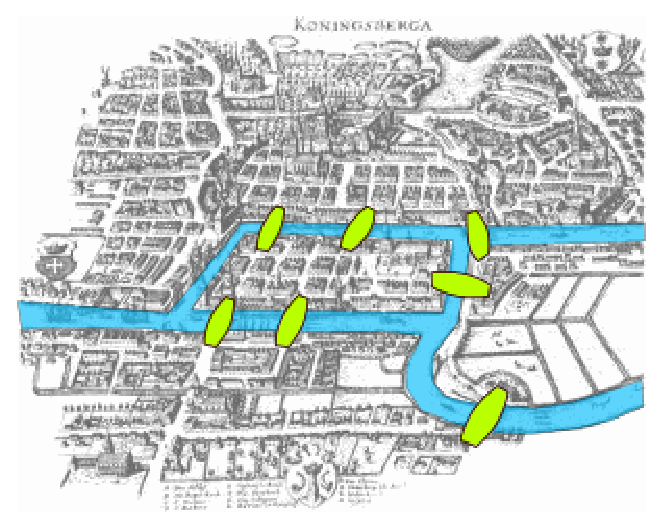
\includegraphics[width=140px]{konigsberg_bridges.eps}\\
			{\footnotesize credit : Wikipedia}
		\end{center}
		\textit{Est-il possible de trouver un chemin qui passe une seule fois par chaque pont ?\\}
        \onslide<2->{\small Ce problème (\textit{problème des sept ponts de Königsberg}) a été étudié par le mathématicien suisse Leonhard Euler en 1736 et est considéré historiquement comme le premier problème faisant intervenir la théorie des graphes.\\}
        \onslide<3->{Les graphes sont maintenant un domaine central de l'informatique ({\sc gps}, réseaux, \dots)}
	\end{block}
\end{frame}

\makess{Graphes orientés}
\begin{frame}[fragile]{\Ctitle}{\stitle}
	\begin{alertblock}{Définition}
		Un \textcolor{red}{graphe orienté} est la donnée :
		\begin{itemize}
			\item<2->{D'un ensemble de \textcolor{blue}{sommets} $S$ (\textcolor{gray}{V pour \textit{vertice} en anglais.}).}
			\item<3->{D'un ensemble de couples de sommets $A \subseteq S \times S$ appelés \textcolor{blue}{arc} (notés $x \rightarrow y$).(\textcolor{gray}{E pour \textit{edges} en anglais}).}
		\end{itemize}
        \onslide<4->{On utilisera souvent la notation $G = (S,A)$ pour désigner un graphe orienté.}
	\end{alertblock}
\end{frame}

% Premiers exemples
\begin{frame}[fragile]{\Ctitle}{\stitle}
	\begin{exampleblock}{Exemple}
		\begin{pspicture}(0,0)(5,4)
			\rput(1,1){\circlenode{S1}{$a$}}
			\rput(2,3){\circlenode{S2}{$b$}}
			\rput(4,2){\circlenode{S3}{$c$}}
			\rput(8,3){\circlenode{S4}{$d$}}
			\rput(7,2){\circlenode{S5}{$e$}}
			\rput(6,3){\circlenode{S6}{$f$}}
			\rput(4,3.5){\circlenode{S7}{$g$}}
			\ncarc{->}{S5}{S6}
			\ncarc{->}{S4}{S5}
			\ncarc{->}{S6}{S4}
			\ncarc{->}{S1}{S2}
			\ncarc{->}{S2}{S1}
			\ncarc{->}{S2}{S3}
			\ncarc{->}{S2}{S7}
		\end{pspicture}\\
		\onslide<2->{$S = \{a,b,c,d,e,f,g\}$ \\}
		\onslide<3->{$A = \{(e,f),(d,e),(f,d),(a,b),(b,a),(b,c),(b,g)\}$\\}
		\onslide<4->{\textcolor{BrickRed}{\small \danger} Seule la données de $S$ et $A$ défini le graphe et \textit{pas} les positions des sommets sur le schéma.}
	\end{exampleblock}
\end{frame}

% Vocabulaire
\begin{frame}[fragile]{\Ctitle}{\stitle}
	\begin{block}{Vocabulaire}
		\begin{itemize}
			\item<1-> Le \textcolor{blue}{ordre} d'un graphe est son nombre de sommets.
			\item<2-> Un arc de la forme $(x,x)$ est une \textcolor{blue}{boucle}.
			\item<2-> Les \textcolor{blue}{successeurs} (ou \textcolor{blue}{voisins sortants}) d'un sommet $s \in S$ sont les éléments de l'ensemble ${\cal V_{+}}(s) = \{t \in S  \text{ tel que } s \to t\}$.
			\item<3-> Le \textcolor{blue}{degré sortant} d'un sommet $s$ noté $d_+(s)$ est son nombre de successeurs $d_+(s) = |{\cal V_+}(s)|$.
			\item<4-> Les \textcolor{blue}{prédecesseurs} (ou \textcolor{blue}{voisins entrants}) d'un sommet $s \in S$ sont les éléments de l'ensemble ${\cal V_{-}}(s) = \{t \in S  \text{ tel que } t \to s\}$.
			\item<5-> Le \textcolor{blue}{degré entrant} d'un sommet $s$ noté $d_-(s)$ est son nombre de prédécesseurs $d_-(s) = |{\cal V_-}(s)|$.
			\item<6-> Les \textcolor{blue}{voisins} d'un sommet $s$ sont les éléments de ${\cal V}(s) = {\cal V_+}(s) \cup {\cal V_-}(s) $
			\item<7-> Le \textcolor{blue}{degré} d'un sommet $s$ noté $d(s)$ est la somme de ses degrés entrants et sortants $d(s) = d_-(s)+d_+(s)$
		\end{itemize}
	\end{block}
\end{frame}

% Exercices

\begin{frame}[fragile]{\Ctitle}{\stitle}
	\begin{exampleblock}{Exemple}
		\vspace{0.2cm}
		\begin{pspicture}(-2,-2)(2,2)
			\rput(0,2){\Circlenode{T1}{$a$}}
			\rput(-1.5,0.9){\Circlenode{T2}{$b$}}
			\rput(1,-1){\Circlenode{T4}{$d$}}
			\rput(-1,-1){\Circlenode{T3}{$c$}}
			\rput(1.5,0.9){\Circlenode{T5}{$e$}}
		\end{pspicture}
		\ncline{->}{T1}{T2}
		\ncline{->}{T2}{T3}
		\ncline{->}{T3}{T4}
		\ncline{->}{T4}{T5}
		\ncline{->}{T5}{T1}
		\ncarc{->}{T1}{T3}
		\ncarc{->}{T1}{T4}
		\ncarc{->}{T4}{T1} \vspace{-0.7cm}
		\begin{itemize}
			\item<2-> $V_+(a)= $ \alt<6->{\textcolor{OliveGreen}{$\{b,c,d\}$}}{?}
			\item<3-> $V_+(d)= $ \alt<7->{\textcolor{OliveGreen}{$\{a,c\}$}}{?}
			\item<4-> $d_+(e)= $  \alt<8->{\textcolor{OliveGreen}{$1$}}{?}
			\item<5-> $d_-(a)= $  \alt<9->{\textcolor{OliveGreen}{$2$}}{?}
		\end{itemize}
	\end{exampleblock}
\end{frame}


\begin{frame}[fragile]{\Ctitle}{\stitle}
	\begin{alertblock}{Définition}
		\onslide<1->{Un \textcolor{red}{graphe non orienté} est la donnée :}
		\begin{itemize}
			\item<2->{D'un ensemble de \textcolor{blue}{sommets ou noeuds} $S$.}
			\item<3->{D'un ensemble de \textbf{paires} de sommets $A$  appelés \textcolor{blue}{arcs ou arêtes} notés $x \text{ --- } y$.}
		\end{itemize}
	\end{alertblock}
	\begin{block}{Vocabulaire}
		\begin{itemize}
			\item<4-> Dans le contexte des graphes orientés cela revient à $(x,y) \in A$ ssi $(y,x) \in A$.
			\item<5-> Les définitions de chemin, degrés, \dots des graphes orientés s'étendent naturellement aux graphes non orientés.
			\item<6-> On dit qu'un graphe non orienté $(S,A)$ est \textcolor{blue}{connexe} lorsqu'il existe un chemin entre toute paire de sommets.
		\end{itemize}
	\end{block}
\end{frame}

%graphes pondérés
\begin{frame}[fragile]{\Ctitle}{\stitle}
	\begin{block}{Graphes pondérés}
		\begin{itemize}
			\item<1-> Dans de nombreuses situations, on est amené à attacher une information aux arcs d'un graphe (ex : distance entre deux villes, coût d'une liaison dans un réseau informatique, \dots), on parle alors de \textcolor{blue}{graphe pondéré}.
			\item<2-> L'information, ou \textcolor{blue}{étiquette} attaché à un noeud est souvent de nature numérique, on parle alors de \textcolor{blue}{poids} ou \textcolor{blue}{longueur} d'un arc.
				\item<3->Le coût d'un chemin est alors la somme des poids des arcs qui le compose.
		\end{itemize}
	\end{block}
	\onslide<4->{
		\begin{exampleblock}{Exemple}
			\begin{pspicture}(0,0)(5,2.2)
				\rput(1,1){\circlenode{A}{$a$}}
				\rput(6,1){\circlenode{B}{$b$}}
				\rput(1,2){\circlenode{C}{$c$}}
				\rput(6,2){\circlenode{D}{$d$}}
				\rput(3.5,1.5){\circlenode{E}{$e$}}
				\ncarc{->}{C}{E} \naput{3}
				\ncarc{->}{A}{E} \nbput{7}
				\ncarc{->}{E}{B} \naput{4}
				\ncarc{->}{B}{D} \nbput{1}
				\ncarc{->}{B}{A} \naput{3}
				\ncarc{->}{C}{A} \nbput{2}
			\end{pspicture}
		\end{exampleblock}}
\end{frame}

% Implémentation des graphes par matrice d'adjacence
\begin{frame}[fragile]{\Ctitle}{\stitle}
	\begin{alertblock}{Représentation par matrice d'adjacence}
		On peut représenter un graphe à $n$ sommets par sa \textcolor{blue}{matrice d'adjacence} $M$, c'est-à-dire un tableau de $n$ lignes et $n$ colonnes :
		\begin{itemize}
			\item<2-> On numérote les sommets du graphe
			\item<3-> S'il y a une arête du sommet $i$ vers le sommet $j$ alors on place un 1 à la ligne $i$ et à la colonne $j$ de $M$
			\item<4-> Sinon on place un 0
		\end{itemize}
	\end{alertblock}
	\begin{block}{Remarques}
		\begin{itemize}
			\item<5-> Si le graphe n'est pas orienté alors la matrice est symétrique par rapport à sa première diagonale.
			\item<6-> On peut représenter les graphes pondérés en écrivant le poids à la place du 1 pour chaque arête.
		\end{itemize}
	\end{block}
\end{frame}

% Exemple de matrice d'adjacences
\begin{frame}[fragile]{\Ctitle}{\stitle}
	\begin{exampleblock}{Exemple}
		\begin{enumerate}
			\item<1-> En supposant les sommets numérotés dans l'ordre alphabétique, écrire la matrice d'adjacence du graphe suivant :
				\begin{center}
					\begin{pspicture}(5,2)
						\rput(0,1.8){\circlenode{A}{A}}
						\rput(1,0.5){\circlenode{E}{E}}
						\rput(2,1){\circlenode{B}{B}}
						\rput(4,0.7){\circlenode{D}{D}}
						\rput(6,1.5){\circlenode{C}{C}}
						\ncarc{->}{A}{E}
						\ncarc{->}{A}{B}
						\ncarc{->}{A}{C}
						\ncarc[arcangle=-10]{->}{B}{D}
						\ncarc{->}{C}{B}
						\ncarc[arcangle=-10]{->}{D}{C}
						\ncarc[arcangleA=-45,arcangleB=-40]{->}{E}{C}
						\ncline{->}{E}{B}
					\end{pspicture}
				\end{center}
			\item<2-> Dessiner le graphe ayant la matrice d'adjacence suivante (on appellera les sommets $S_1, S_2, \dots $) :\\
				$\begin{pmatrix}
						0 & 0 & 1 & 1 & 1 \\
						1 & 0 & 1 & 0 & 0 \\
						1 & 1 & 0 & 0 & 1 \\
						1 & 0 & 0 & 1 & 0 \\
						0 & 0 & 1 & 0 & 0 \\
					\end{pmatrix}$
		\end{enumerate}
	\end{exampleblock}
\end{frame}


% Implémentation des graphes par liste d'adjacence
\begin{frame}[fragile]{\Ctitle}{\stitle}
	\begin{alertblock}{Représentation par listes d'adjacence}
		On peut représenter un graphe à l'aide de listes d'adjacences, c'est-à-dire en mémorisant pour chaque sommet du graphe la liste de ses voisins.
		\begin{itemize}
			\item<2-> On crée pour chaque sommet du graphe une liste
			\item<3-> S'il y a une arête du sommet $S_i$ vers le sommet $S_j$ alors  $S_j$ est dans la liste de $S_i$
		\end{itemize}
	\end{alertblock}
	\begin{block}{Remarques}
		\begin{itemize}
			\item<5-> Lorsqu'un graphe a "peu" d'arête cette implémentation est plus intéressante en terme d'occupation mémoire que celle par matrice d'adjacence.
			\item<6-> En Python, on utilisera un dictionnaire pour représenter les listes d'adjacences, les clés sont les sommets et les valeurs les listes associées
		\end{itemize}
	\end{block}
\end{frame}

% Exemple de liste d'adjacences
\begin{frame}[fragile]{\Ctitle}{\stitle}
	\begin{exampleblock}{Exemple}
		\begin{enumerate}
			\item<1-> Ecrire les listes d'adjacences du graphe suivante :
			\begin{center}
				\begin{pspicture}(5,2)
					\rput(0,1.8){\circlenode{A}{A}}
					\rput(1,0.5){\circlenode{E}{E}}
					\rput(2,1){\circlenode{B}{B}}
					\rput(4,0.7){\circlenode{D}{D}}
					\rput(6,1.5){\circlenode{C}{C}}
					\ncarc{->}{A}{E}
					\ncarc{->}{A}{B}
					\ncarc{->}{A}{C}
					\ncarc[arcangle=-10]{->}{B}{D}
					\ncarc{->}{C}{B}
					\ncarc[arcangle=-10]{->}{D}{C}
					\ncarc[arcangleA=-45,arcangleB=-40]{->}{E}{C}
					\ncline{->}{E}{B}
				\end{pspicture}
			\end{center}
			\item<2-> Dessiner le graphe représenté par le dictionnaire Python suivante :
				\begin{lstlisting}
{ 	
	'A' : ['C'],
 	'B' : ['D','E'],
 	'C' : ['A','B'],
 	'D' : ['A','C'],
 	'E' : ['B','C','D']
} 
\end{lstlisting}
		\end{enumerate}
	\end{exampleblock}
\end{frame}

% Exemple de matrice d'adjacences
\begin{frame}[fragile]{\Ctitle}{\stitle}
	\begin{block}{Parcours d'un graphe}
		A la base des algorithmes sur les graphes, on trouve les parcours de graphe, c'est-à-dire l'exploration des sommets. A partir du sommet de départ, on peut :
		\begin{itemize}
			\item<1-> explorer tous ses voisins immédiats, puis les voisins des voisins et ainsi de suite. Le graphe est donc exploré en \og cercle concentrique\fg autour du sommet de départ  \dots, on parle alors de  \textcolor{blue}{parcours en largeur} ou \textcolor{gray}{breadth first search (\textit{BFS})} en anglais.
			\item<2-> explorer à chaque étape le premier voisin non encore exploré. Lorsque qu'on atteint un sommet dont tous les voisins ont déjà été exploré, on revient en arrière, on parle alors de  \textcolor{blue}{parcours en profondeur} ou \textcolor{gray}{depth first search (\textit{DFS})} en anglais.
		\end{itemize}
	\end{block}
\end{frame}

% Parcours en largeur
\begin{frame}[fragile]{\Ctitle}{\stitle}
	\begin{exampleblock}{Exemple de parcours en largeur}
		\begin{center}
			\begin{pspicture}(5,2)
				\alt<2->{\rput(0,1.8){\visited{A}}}{\rput(0,1.8){\normal{A}}}
				\alt<3->{\rput(1,0.5){\visited{E}}}{\rput(1,0.5){\normal{E}}}
				\alt<3->{\rput(2,1){\visited{B}}}{\rput(2,1){\normal{B}}}
				\alt<3->{\rput(6,1.5){\visited{C}}}{\rput(6,1.5){\normal{C}}}
				\alt<5->{\rput(6,0){\visited{F}}}{\rput(6,0){\normal{F}}}
				\alt<7->{\rput(7,0.7){\visited{G}}}{\rput(7,0.7){\normal{G}}}
				\alt<5->{\rput(4,0.7){\visited{D}}}{\rput(4,0.7){\normal{D}}}
				\ncarc{->}{A}{E}
				\ncarc{->}{A}{B}
				\ncarc{->}{A}{C}
				\ncarc[arcangle=-10]{->}{B}{D}
				\ncarc{->}{C}{B}
				\ncarc[arcangle=-10]{->}{C}{F}
				\ncarc[arcangle=-10]{->}{F}{G}
				\ncarc[arcangle=-10]{->}{D}{C}
				\ncarc[arcangleA=-45,arcangleB=-40]{->}{E}{C}
				\ncline{->}{E}{B}
			\end{pspicture}
		\end{center} \vspace{0.2cm}
		Sommets explorés  : \onslide<2->{\fbox{A,}} \onslide<4->{\fbox{B, C, E}} \onslide<6->{\fbox{D, F,}} \onslide<8->{\fbox{G\phantom{,}}} \\
		\onslide<9->{Ecrire le parcours en largeur du graphe suivant (on part du sommet $S_1$)
			\begin{pspicture}(0,-1.6)(5,1.6)
				\rput(1,1.3){\circlenode{R1}{$S_1$}}
				\rput(3,1.3){\circlenode{R2}{$S_2$}}
				\rput(1,0){\circlenode{R3}{$S_3$}}
				\rput(3,0){\circlenode{R4}{$S_4$}}
				\rput(5,0){\circlenode{R5}{$S_5$}}
				\rput(1,-1.3){\circlenode{R6}{$S_6$}}
				\rput(3,-1.3){\circlenode{R7}{$S_7$}}
				\rput(5,-1.3){\circlenode{R8}{$S_8$}}
				\ncline{->}{R1}{R2}
				\ncline{->}{R2}{R4}
				\ncline{->}{R2}{R5}
				\ncline{->}{R4}{R6}
				\ncline{->}{R4}{R7}
				\ncline{->}{R6}{R3}
				\ncline{->}{R4}{R1}
				\ncline{->}{R4}{R5}
				\ncline{->}{R7}{R8}
				\ncline{->}{R8}{R5}
				\ncline{->}{R3}{R1}
			\end{pspicture}}
	\end{exampleblock}
\end{frame}

% Ex parcours en profondeur
\begin{frame}[fragile]{\Ctitle}{\stitle}
	\begin{exampleblock}{Exemple de parcours en profondeur}
		\begin{center}
			\begin{pspicture}(5,2)
				\alt<2->{\rput(0,1.8){\visited{A}}}{\rput(0,1.8){\normal{A}}}
				\alt<3->{\rput(2,1){\visited{B}}}{\rput(2,1){\normal{B}}}
				\alt<5->{\rput(6,1.5){\visited{C}}}{\rput(6,1.5){\normal{C}}}
				\alt<4->{\rput(4,0.7){\visited{D}}}{\rput(4,0.7){\normal{D}}}
				\alt<8->{\rput(1,0.5){\visited{E}}}{\rput(1,0.5){\normal{E}}}
				\alt<6->{\rput(6,0){\visited{F}}}{\rput(6,0){\normal{F}}}
				\alt<7->{\rput(7,0.7){\visited{G}}}{\rput(7,0.7){\normal{G}}}
				\ncarc{->}{A}{E}
				\ncarc{->}{A}{B}
				\ncarc{->}{A}{C}
				\ncarc[arcangle=-10]{->}{B}{D}
				\ncarc{->}{C}{B}
				\ncarc[arcangle=-10]{->}{C}{F}
				\ncarc[arcangle=-10]{->}{F}{G}
				\ncarc[arcangle=-10]{->}{D}{C}
				\ncarc[arcangleA=-45,arcangleB=-40]{->}{E}{C}
				\ncline{->}{E}{B}
			\end{pspicture}
		\end{center} \vspace{0.2cm}
		Sommets explorés  : \onslide<2->{A,} \onslide<3->{B,} \onslide<4->{D,} \onslide<5->{C,} \onslide<6->{F,} \onslide<7->{G,} \onslide<8->{E} \\
		\onslide<9->{Ecrire le parcours en profondeur du graphe suivant (on part du sommet $S_1$)
			\begin{pspicture}(0,-1.6)(5,1.6)
				\rput(1,1.3){\circlenode{R1}{$S_1$}}
				\rput(3,1.3){\circlenode{R2}{$S_2$}}
				\rput(1,0){\circlenode{R3}{$S_3$}}
				\rput(3,0){\circlenode{R4}{$S_4$}}
				\rput(5,0){\circlenode{R5}{$S_5$}}
				\rput(1,-1.3){\circlenode{R6}{$S_6$}}
				\rput(3,-1.3){\circlenode{R7}{$S_7$}}
				\rput(5,-1.3){\circlenode{R8}{$S_8$}}
				\ncline{->}{R1}{R2}
				\ncline{->}{R2}{R4}
				\ncline{->}{R2}{R5}
				\ncline{->}{R4}{R6}
				\ncline{->}{R4}{R7}
				\ncline{->}{R6}{R3}
				\ncline{->}{R4}{R1}
				\ncline{->}{R4}{R5}
				\ncline{->}{R7}{R8}
				\ncline{->}{R8}{R5}
				\ncline{->}{R3}{R1}
			\end{pspicture}}
	\end{exampleblock}
\end{frame}

\begin{frame}[fragile]{\Ctitle}{\stitle}
	\begin{block}{File et parcours en largeur}
		\begin{itemize}
			\item<1-> Pour un parcours en largeur, on doit stocker dans une structure de données les sommets en attente d'être explorés. c'est-à-dire les voisins du sommet de départ, puis les voisins des voisins \dots 
			Ces sommets doivent être retirés pour exploration, \textit{dans leur ordre d'insertion}, la structure de données utilisée est donc du type \textcolor{blue}{premier entré, premier sorti} (\textcolor{gray}{first in first out : \textit{\sc fifo}}).
			\item<2-> Ce type de structure de données s'appelle une \textcolor{blue}{file}.
			\item<3-> Pour l'implémentation on doit pouvoir \textcolor{blue}{enfiler} (ajouter un sommet dans la file) et \textcolor{blue}{défiler} (retirer un sommet) de façon efficace donc en $\mathcal{O}(1)$. 
			\item<4-> Les listes de Python ne sont pas adaptées, on utilisera le module \kw{deque} de Python, enfiler correspond alors à \kw{appendleft} et défiler à \kw{pop}.\vspace{0.4cm} \\
			\onslide<5->{\rnode{enf}{\framebox[1cm]{$F$}}}  \hspace{2cm}
			\begin{tabular}{|p{0.5cm}|p{0.5cm}|p{0.5cm}|p{0.5cm}|}
				\hline
				\rnode{in}{$E$} & {$D$} & {$C$} & \rnode{out}{$B$} \\
				\hline
				\multicolumn{4}{c}{File d'attente} \\
			\end{tabular}
			\hspace{2cm} \onslide<9->{\rnode{def}{\framebox[1cm]{$B$}}}
			\onslide<5->{\ncline[linestyle=dashed,nodesepB=0.2cm]{->}{enf}{in}}
			\onslide<6->{\naput{{\footnotesize \textcolor{blue}{{\tt appendleft}}}}}
			\onslide<9->{\ncline[linestyle=dashed,nodesepA=0.4cm]{->}{out}{def}}
			\onslide<10->{\naput{{\footnotesize \textcolor{blue}{\tt pop}}}}
		\end{itemize}
	\end{block}
\end{frame}

\begin{frame}[fragile]{\Ctitle}{\stitle}
	\begin{block}{File et parcours en profondeur}
		\begin{itemize}
			\item<1-> Pour un parcours en profondeur, on stocker aussi dans une structure de données les sommets en attente d'être explorés. Mais cette fois, la structure de données utilisée est donc du type \textcolor{blue}{dernier entré, premier sorti} (\textcolor{gray}{last in first out (\textit{\sc lifo})}).
			\item<2-> Ce type de structure de données s'appelle une \textcolor{blue}{pile}.
			\item<3-> Pour l'implémentation, on se contente d'utiliser la récursivité de façon à ce que la pile des sommets en attente d'être exploré soit gérée de façon automatique par les appels récursifs.
		\end{itemize}
	\end{block}
\end{frame}

\begin{frame}[fragile]{\Ctitle}{\stitle}
	\begin{exampleblock}{Algorithme de Djikstra : exemple}
		\begin{center}
			\begin{pspicture}(5,2.7)
				\rput(0,2.2){\circlenode[linewidth=1pt,linecolor=red,fillcolor=fluo,fillstyle=solid]{A}{A}}
				\alt<15->{\rput(5,1.2){\circlenode[linewidth=1pt,linecolor=red,fillcolor=fluo,fillstyle=solid]{E}{E}}}{\rput(5,1.2){\circlenode{E}{E}}}
				\alt<11->{\rput(1.5,1.1){\circlenode[linewidth=1pt,linecolor=red,fillcolor=fluo,fillstyle=solid]{B}{B}}}{\rput(1.5,1.1){\circlenode{B}{B}}}
				\alt<22->{\rput(4,0.4){\circlenode[linewidth=1pt,linecolor=red,fillcolor=fluo,fillstyle=solid]{D}{D}}}{\rput(4,0.4){\circlenode{D}{D}}}
				\alt<6->{\rput(3,2.3){\circlenode[linewidth=1pt,linecolor=red,fillcolor=fluo,fillstyle=solid]{C}{C}}}{\rput(3,2.3){\circlenode{C}{C}}}
				\alt<19->{\rput(7,1.3){\circlenode[linewidth=1pt,linecolor=red,fillcolor=fluo,fillstyle=solid]{F}{F}}}{\rput(7,1.3){\circlenode{F}{F}}}
				\alt<5->{\ncarc[linecolor=red,linewidth=1pt]{A}{C}}{\ncarc{A}{C}} \naput{1}
				\alt<4->{\ncarc[arcangle=-10,linecolor=red,linewidth=1pt]{A}{B}}{\ncarc[arcangle=-10]{A}{B}} \naput{5}
				\alt<8->{\ncarc[linecolor=red,linewidth=1pt]{B}{C}}{\ncarc{B}{C}} \naput{3}
				\alt<14->{\ncarc[linewidth=1pt,linecolor=red]{B}{E}}{\ncarc{B}{E}} \naput{2}
				\alt<10->{\ncarc[linecolor=red,linewidth=1pt]{C}{F}}{\ncarc{C}{F}} \naput{7}
				\alt<9->{\ncarc[arcangle=-5,linecolor=red,linewidth=1pt]{C}{E}}{\ncarc[arcangle=-5]{C}{E}} \naput{5}
				\alt<13->{\ncarc[arcangle=-10,linecolor=red,linewidth=1pt]{B}{D}}{\ncarc[arcangle=-10]{B}{D}} \nbput{4}
				\alt<21->{\ncarc[arcangle=-10,linecolor=red,linewidth=1pt]{D}{F}}{\ncarc[arcangle=-10]{D}{F}} \nbput{3}
				\alt<18->{\ncarc[linecolor=red,linewidth=1pt]{E}{F}}{\ncarc{E}{F}} \naput{1}
			\end{pspicture}
		\end{center}
		\begin{tabularx}{\textwidth}{|X|X|X|X|X|X|X|}
			\hline
			A                                        & B                                         & C                                        & D                                      & E                                         & F                                         &                                    \\
			\hline
			\alt<2->{ 0 (A)}{ }                      & \alt<4->{5 (A)}{}                         & \alt<5->{1 (A)}{ }                       &                                        &                                           &                                           & \alt<3->{ \textcolor{blue}{A}}{ }  \\
			\hline
			\alt<3->{\textcolor{blue}{\ding{52}}}{ } & \alt<8->{4 (C)}{ }                        & \alt<6->{\textcolor{red}{1 (A)}}{ }      &                                        & \alt<9->{6 (C)}{ }                        & \alt<10->{8 (C)}{ }                       & \alt<7->{ \textcolor{blue}{C}}{ }  \\
			\hline
			\alt<3->{\textcolor{blue}{\ding{52}}}{ } & \alt<11->{\textcolor{red}{4 (C)}}{ }      & \alt<7->{\textcolor{blue}{\ding{52}}}{ } & \alt<13->{8 (B)}{ }                    & \alt<14->{6 (B)}{ }                       &                     & \alt<12->{ \textcolor{blue}{B}}{ } \\
			\hline
			\alt<3->{\textcolor{blue}{\ding{52}}}{ } & \alt<12->{\textcolor{blue}{\ding{52}}}{ } & \alt<7->{\textcolor{blue}{\ding{52}}}{ } &                  & \alt<15->{\textcolor{red}{6 (B)}}{ }      & \alt<18->{7 (E)}{}                        & \alt<16->{ \textcolor{blue}{E}}{ } \\
			\hline
			\alt<3->{\textcolor{blue}{\ding{52}}}{ } & \alt<12->{\textcolor{blue}{\ding{52}}}{ } & \alt<7->{\textcolor{blue}{\ding{52}}}{ } & \alt<21->{11 (F)}{ }                    & \alt<16->{\textcolor{blue}{\ding{52}}}{ } & \alt<19->{\textcolor{red}{7 (E)}}{ }      & \alt<20->{ \textcolor{blue}{F}}{ } \\
			\hline
			\alt<3->{\textcolor{blue}{\ding{52}}}{ } & \alt<12->{\textcolor{blue}{\ding{52}}}{ } & \alt<7->{\textcolor{blue}{\ding{52}}}{ } & \alt<22->{\textcolor{red}{{8 (B)}}}{ } & \alt<16->{\textcolor{blue}{\ding{52}}}{ } & \alt<19->{\textcolor{blue}{\ding{52}}}{ } & \alt<23->{ \textcolor{blue}{D}}{ } \\
			\hline
		\end{tabularx}
	\end{exampleblock}
\end{frame}

\end{document}

